\section{Research Questions and Hypotheses}

There is a general lack of research into the VR head collisions problem. Current VR developers experiment with various solutions in their games, and all of these methods have their advantages and disadvantages. There is a disagreement in VR developers community over which solution should be used in future games. Some developers wonder if it is even worth the effort to implement any solution at all. Therefore, the goal of this study is to examine different solutions and to determine which one of them is best suited for modern VR games.
 
There are several possible solutions to the VR head collisions problem, and they can be implemented in many different ways. Due to time constraints, only the following four most popular methods were chosen for this study:

\begin{itemize}
\item Screen fade: When the head collision is detected, the whole screen fades to black in the span of a second. The view remains blacked-out for as long as the player's head collides with the object.
\item Delayed push-back: If the player keeps colliding with the object for longer than a second, he is slowly pushed backwards until he leaves the object's boundaries.
\item Instant push-back: When the user starts to collide with some obstacle, a collision vector is computed and its projection on the horizontal plane is immediately added to the player's position.
\item Teleportation: If the collision is detected and maintained for the duration of one second, the player is instantly teleported to the last know valid position. 
\end{itemize}

The quality of VR experience is affected by many factors. VR sickness, the sense of presence in virtual world, and the usability of the user interface are some of the main considerations in designing comfortable VR experience. Some developers consider different factors to be more important than others. For this reason, the proposed solutions to the VR head collisions problem are examined from three different perspectives. The answers to the following research questions will help VR developers decide which particular solution to use:

\begin{itemize}
\item RQ1: How the proposed solutions to the VR head collisions problem affect the virtual reality sickness?
\item RQ2: How the proposed solutions to the VR head collisions problem affect the sense of presence?
\item RQ3: How usable are the proposed solutions to the VR head collisions problem?
\end{itemize}

The three null hypotheses corresponding to the research questions are as follows:

\begin{itemize}
\item H$_{\text{01}}$: All proposed solutions to the VR head collisions problem have the same effect on the virtual reality sickness.
\item H$_{\text{02}}$: All proposed solutions to the VR head collisions problem have the same effect on the sense of presence.
\item H$_{\text{03}}$: All proposed solutions to the VR head collisions problem have the same level of usability.
\end{itemize}

The null hypotheses are tested against the following three alternative hypotheses:

\begin{itemize}
\item H$_{\text{A1}}$: Some proposed solutions to the VR head collisions problem have more positive effect than others on the virtual reality sickness.
\item H$_{\text{A2}}$: Some solutions to the VR head collisions problem have more positive effect than others on the sense of presence.
\item H$_{\text{A3}}$: Some solutions to the VR head collisions problem have higher level of usability than others.
\end{itemize}

\section{Questionnaires}

Two questionnaires were prepared for the study. Before the experiment began, participants were asked to fill in a demographic questionnaire. It included information about age, gender, previous experience with VR, and previous experience with motion sickness (see Appendix A). Each time after testing one of the solutions to the VR head collisions problem, the participants filled in a post-test questionnaire (see Appendix B). This questionnaire is composed of three sections, which correspond accordingly to the three research questions. First, the participants described what VR sickness symptoms they felt during the experiment (see question 2 in Appendix B). Next, they answered to six questions about the sense of presence in the virtual environment (see questions 3-8 in Appendix B). Finally, the participants rated the tested method with eight usability factors on the scale from 1 to 5 (see question 9 in Appendix B).

\subsection{Simulator Sickness Questionnaire}

The VR sickness section of post-test questionnaire was prepared using the Simulator Sickness Questionnaire (SSQ) \cite{SSQ}, a widely acknowledged standard for studying simulator sickness. The SSQ was developed in 1993 with the purpose of enhancing training efficiency in flight simulators. Due to the similarity of simulator sickness with VR sickness, in the recent years the SSQ was also used by many researchers studying comfortable VR locomotion \cite{TELEPORTATIONEFFECTS}\cite{NODEBASEDTELEPORTATION}\cite{SUSMETHODARTICLE}. The SSQ consists of 16 most commonly occurring simulator sickness symptoms: general discomfort, fatigue, headache, eye strain, difficulty focusing, salivation increasing, sweating, nausea, difficulty concentrating, "fullness of the head", blurred vision, dizziness with eyes open, dizziness with eyes closed, vertigo, stomach awareness, and burping. These symptoms fall into three different categories: nausea-related, oculomotor-related, and disorientation-related. Each questionnaire item is scored on a four point scale (0-3): none, slight, moderate, and severe. The scores for each category and the total SSQ score are multiplied by the following weight factors: nausea is multiplied by 9.54, oculomotor by 7.58, disorientation by 13.92, and total SSQ by 3.74.

\subsection{Presence Questionnaire}

The Slayer-Usoh-Steed (SUS) \cite{SUS} presence questionnaire was used to prepare the second section of post-test questionnaire. It was chosen for this study because it is the second most cited presence questionnaire applicable for VR \cite{SUSEVIDENCE}, and it has a relatively short list of six questions in comparison to other, longer questionnaires. All SUS questions are based on one of the three themes: the extent to which the virtual environment becomes the dominant reality, the sense of being in the virtual environment, and the extent to which the virtual environment is remembered as a ``place''. Each question is answered on a scale from 1 to 7, where the higher score indicates greater sense of presence. The final presence score is a number of answers that have a score of 6 or 7.

\subsection{Usability Questionnaire}

In the usability section, the participants rated eight different factors: difficulty in understanding the method, difficulty in operating the method, feeling of being in control while using the method, required effort to use the method, feeling of tiredness while using the method, feeling of enjoyment while using the method, feeling of being overwhelmed while using the method, feeling of frustration while using the method. This exact approach was also used in two recent VR locomotion studies \cite{TELEPORTATIONSTUDY}\cite{NODEBASEDTELEPORTATION}. Each question was answered on a 5 point Likert scale, where 1 meant ``not at all'' and 5 meant ``very much''. The total usability score was calculated as follows: for each factor, except for the ``feeling of being in control'' and ``feeling of enjoyment'', the score was firstly subtracted from 5, and then it was added to the total score. In the two mentioned cases, the factor score was firstly subtracted by 1, and then it was added to the total score.

\section{Implementation}

Opis narzędzi wykorzystanych do implementacji (Unity, VRTK, SteamVR).

\subsection{Virtual Environment}

Opis i zdjęcia wirtualnej sceny, w której będzie odbywa się eksperyment. Scena składa się z 10 różnych przedmiotów (meble, przedmioty, ściany). Scena dla każdej testowanej metody wygląda tak samo. Zmienia się tylko obsługa kolizji na jedną z czterech metod. Użytkownik aby ukończyć eksperyment musi skolidować głową z każdym z przedmiotów na scenie. Przedmioty, z którymi nie odbyła się jeszcze kolizja są podwietlone na zielony kolor. Po zakończeniu testowania metody, użytkownik ściąga VR headset, wypełnia ankietę i następnia rozpoczyna kolejny test. Scena w tym momencie jest zresetowana i używana jest inna obsługa kolizji.

\begin{figure}[th]
\centering
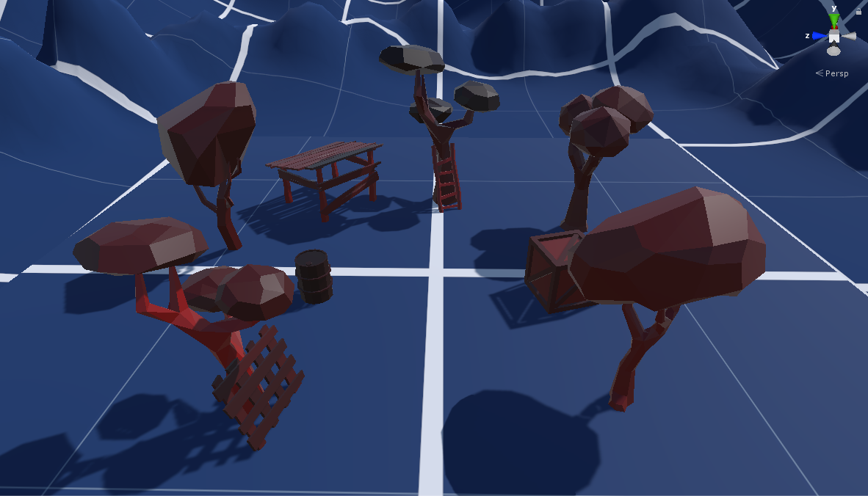
\includegraphics[width=1\textwidth]{img/virtual_environment.png}
\caption{Time slice example of the screen fade technique. When the head collision is detected, the screen slowly fades to black (image source: \cite{SCREENFADE})}
\label{fig:veimplementation}
\end{figure}

\subsection{Screen Fade}

Opis implementacji i zdjęcia zaimplementowanej metody Screen Fade.

\subsection{Object Fade}

Opis implementacji i zdjęcia zaimplementowanej metody Object Fade.

\subsection{Camera Collider}

Opis implementacji i zdjęcia zaimplementowanej metody Camera Collider.

\subsection{Camera Push-Back}

Opis implementacji i zdjęcia zaimplementowanej metody Camera Push-Back.

\begin{figure}[th]
\centering
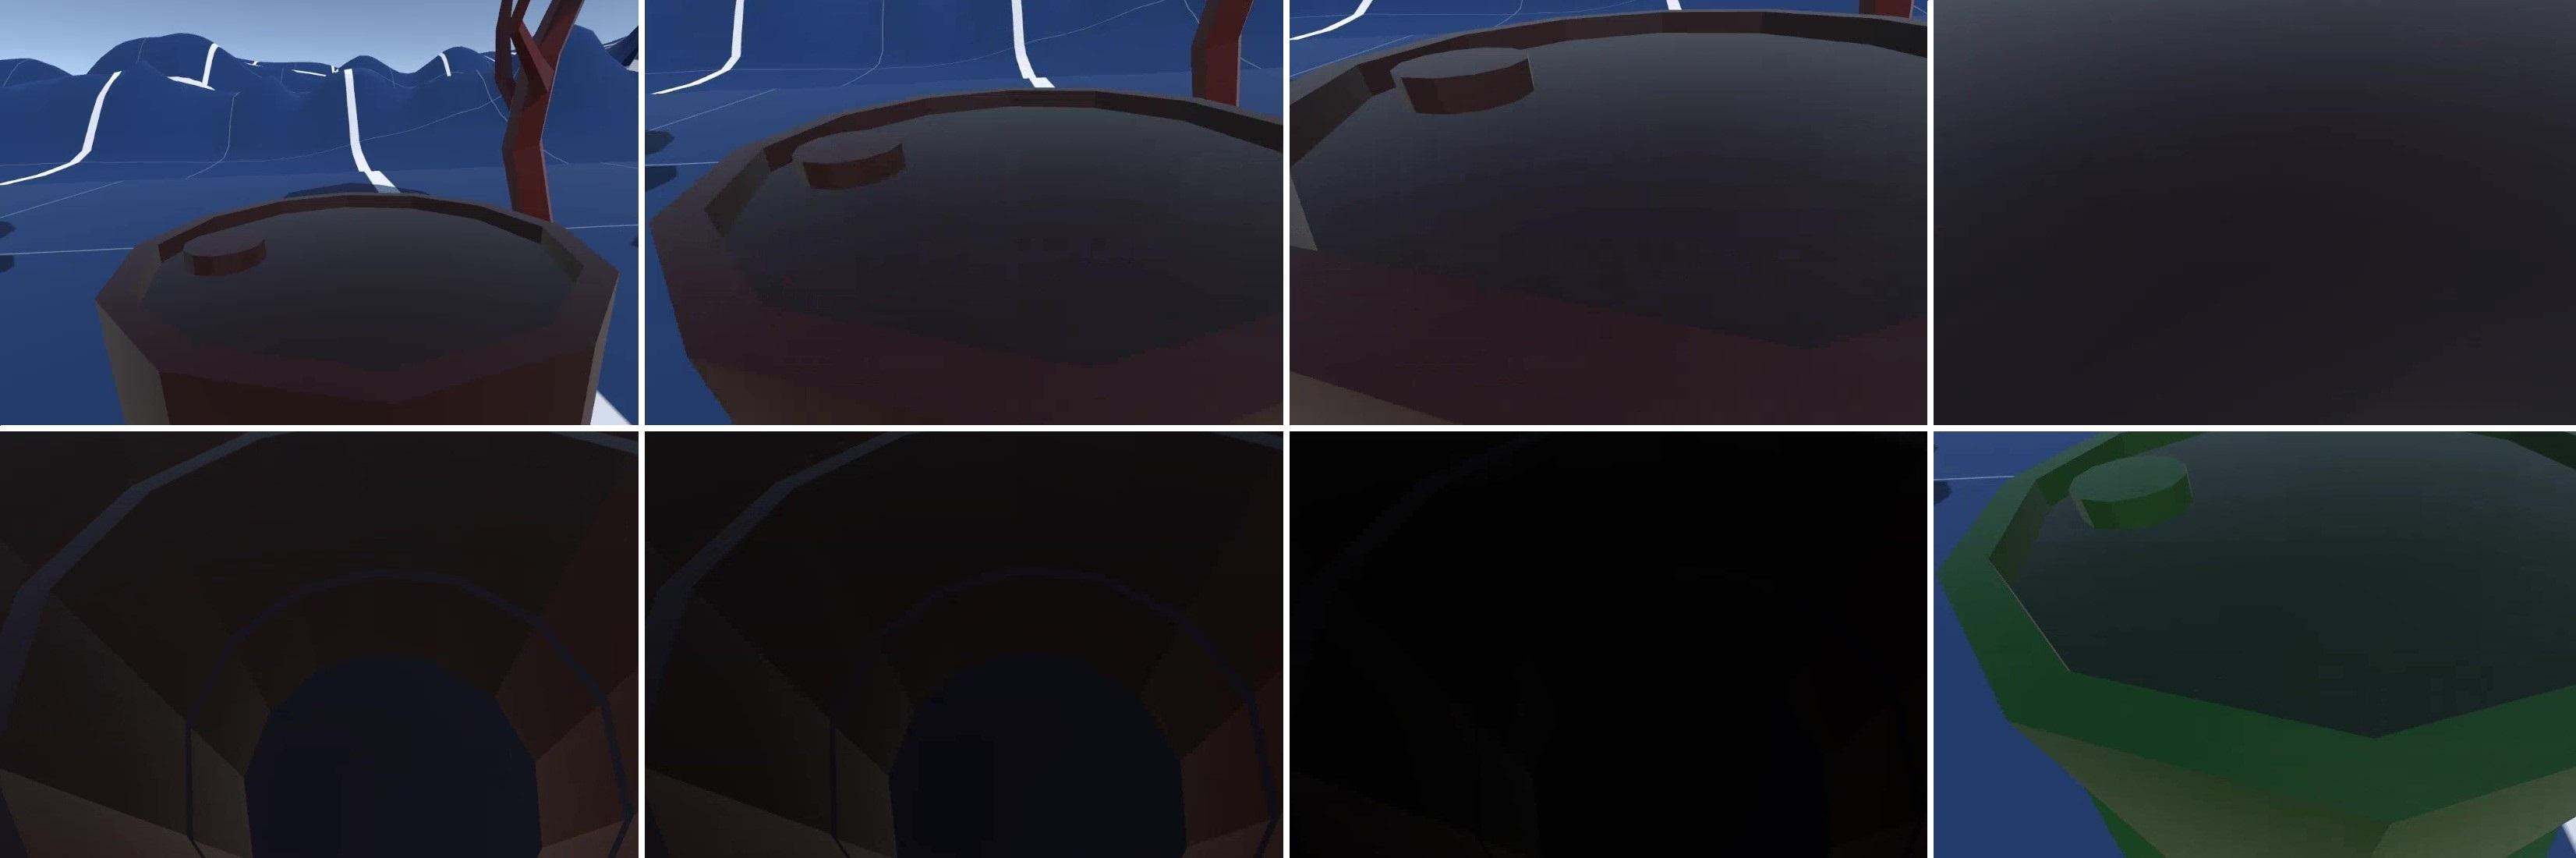
\includegraphics[width=1\textwidth]{img/teleport_implementation.jpg}
\caption{Time slice example of the screen fade technique. When the head collision is detected, the screen slowly fades to black (image source: \cite{SCREENFADE})}
\label{fig:teleportimplementation}
\end{figure}

\begin{figure}[th]
\centering
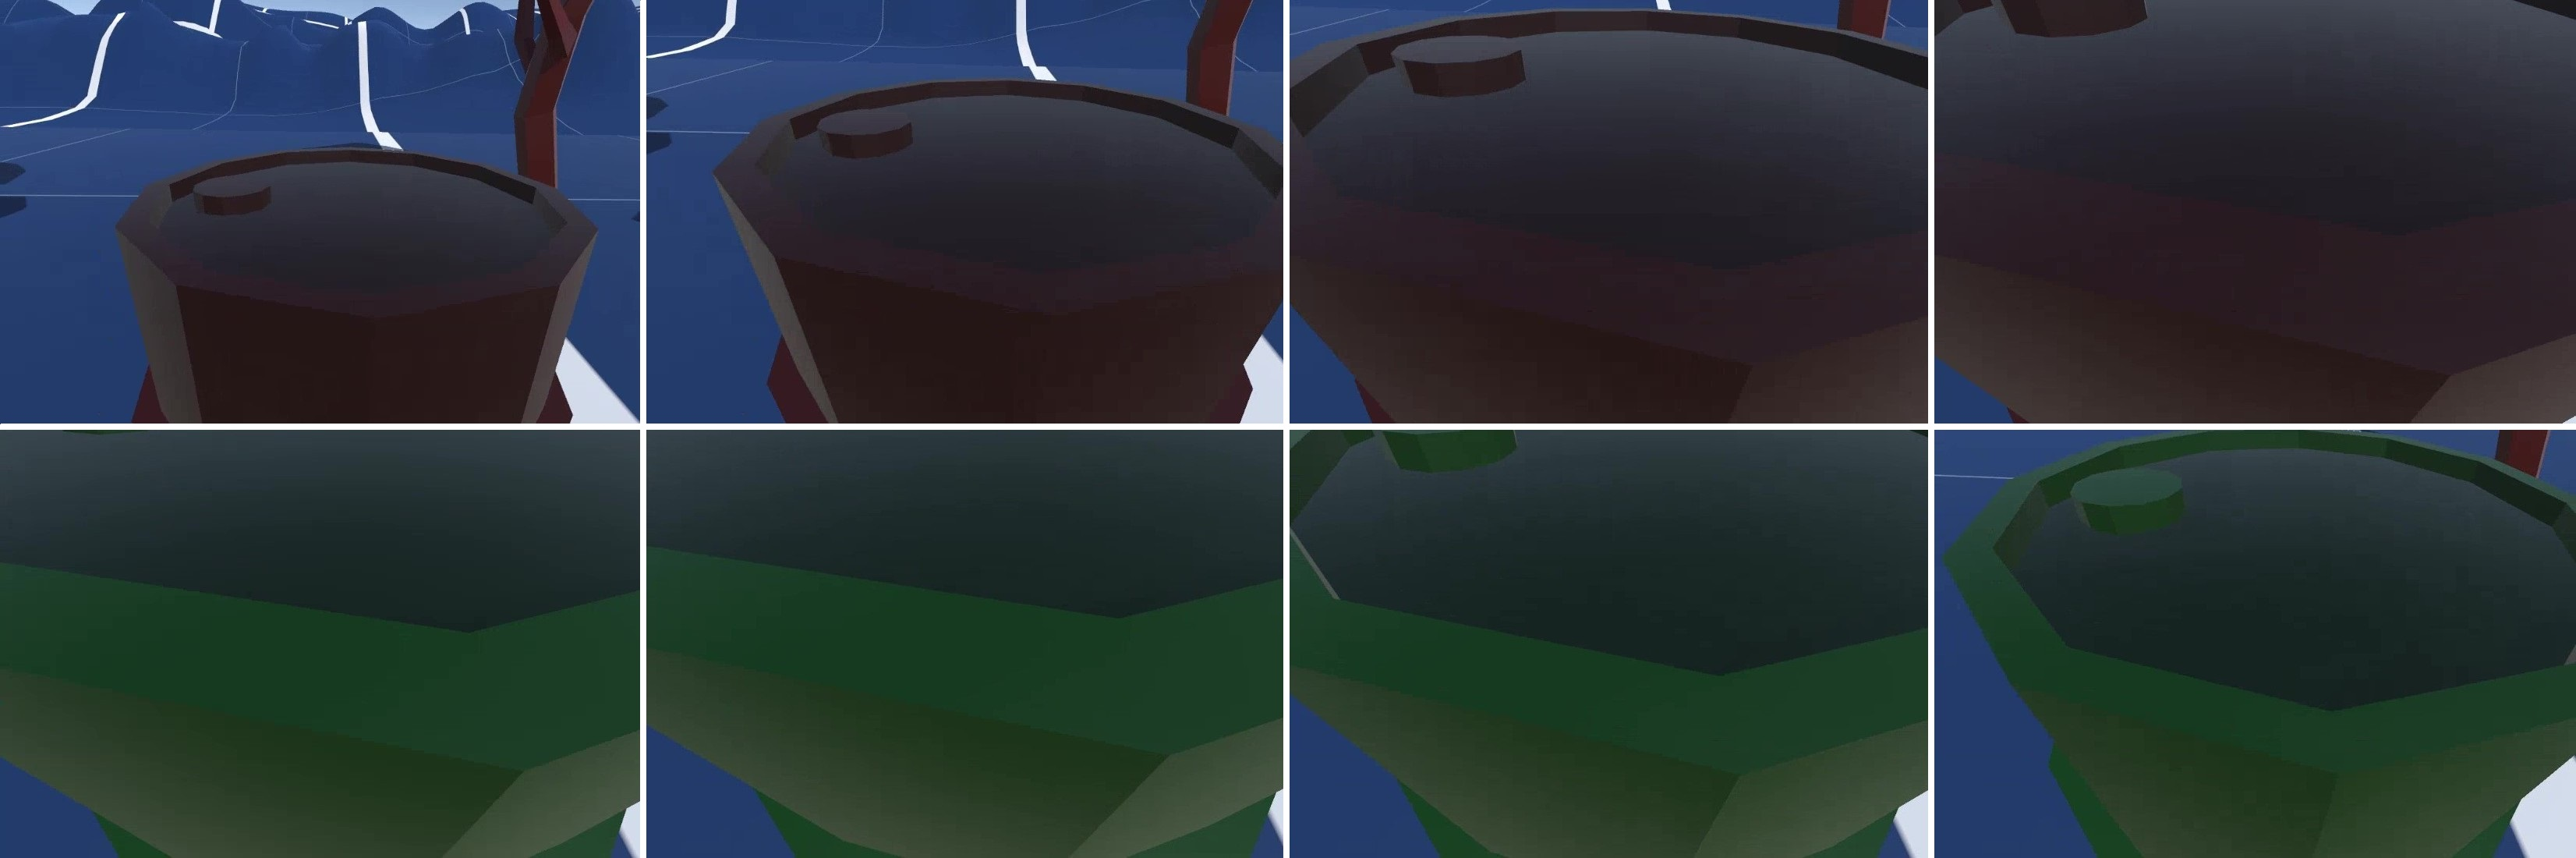
\includegraphics[width=1\textwidth]{img/instant_implementation.jpg}
\caption{Time slice example of the screen fade technique. When the head collision is detected, the screen slowly fades to black (image source: \cite{SCREENFADE})}
\label{fig:instantimplementation}
\end{figure}

\begin{figure}[th]
\centering
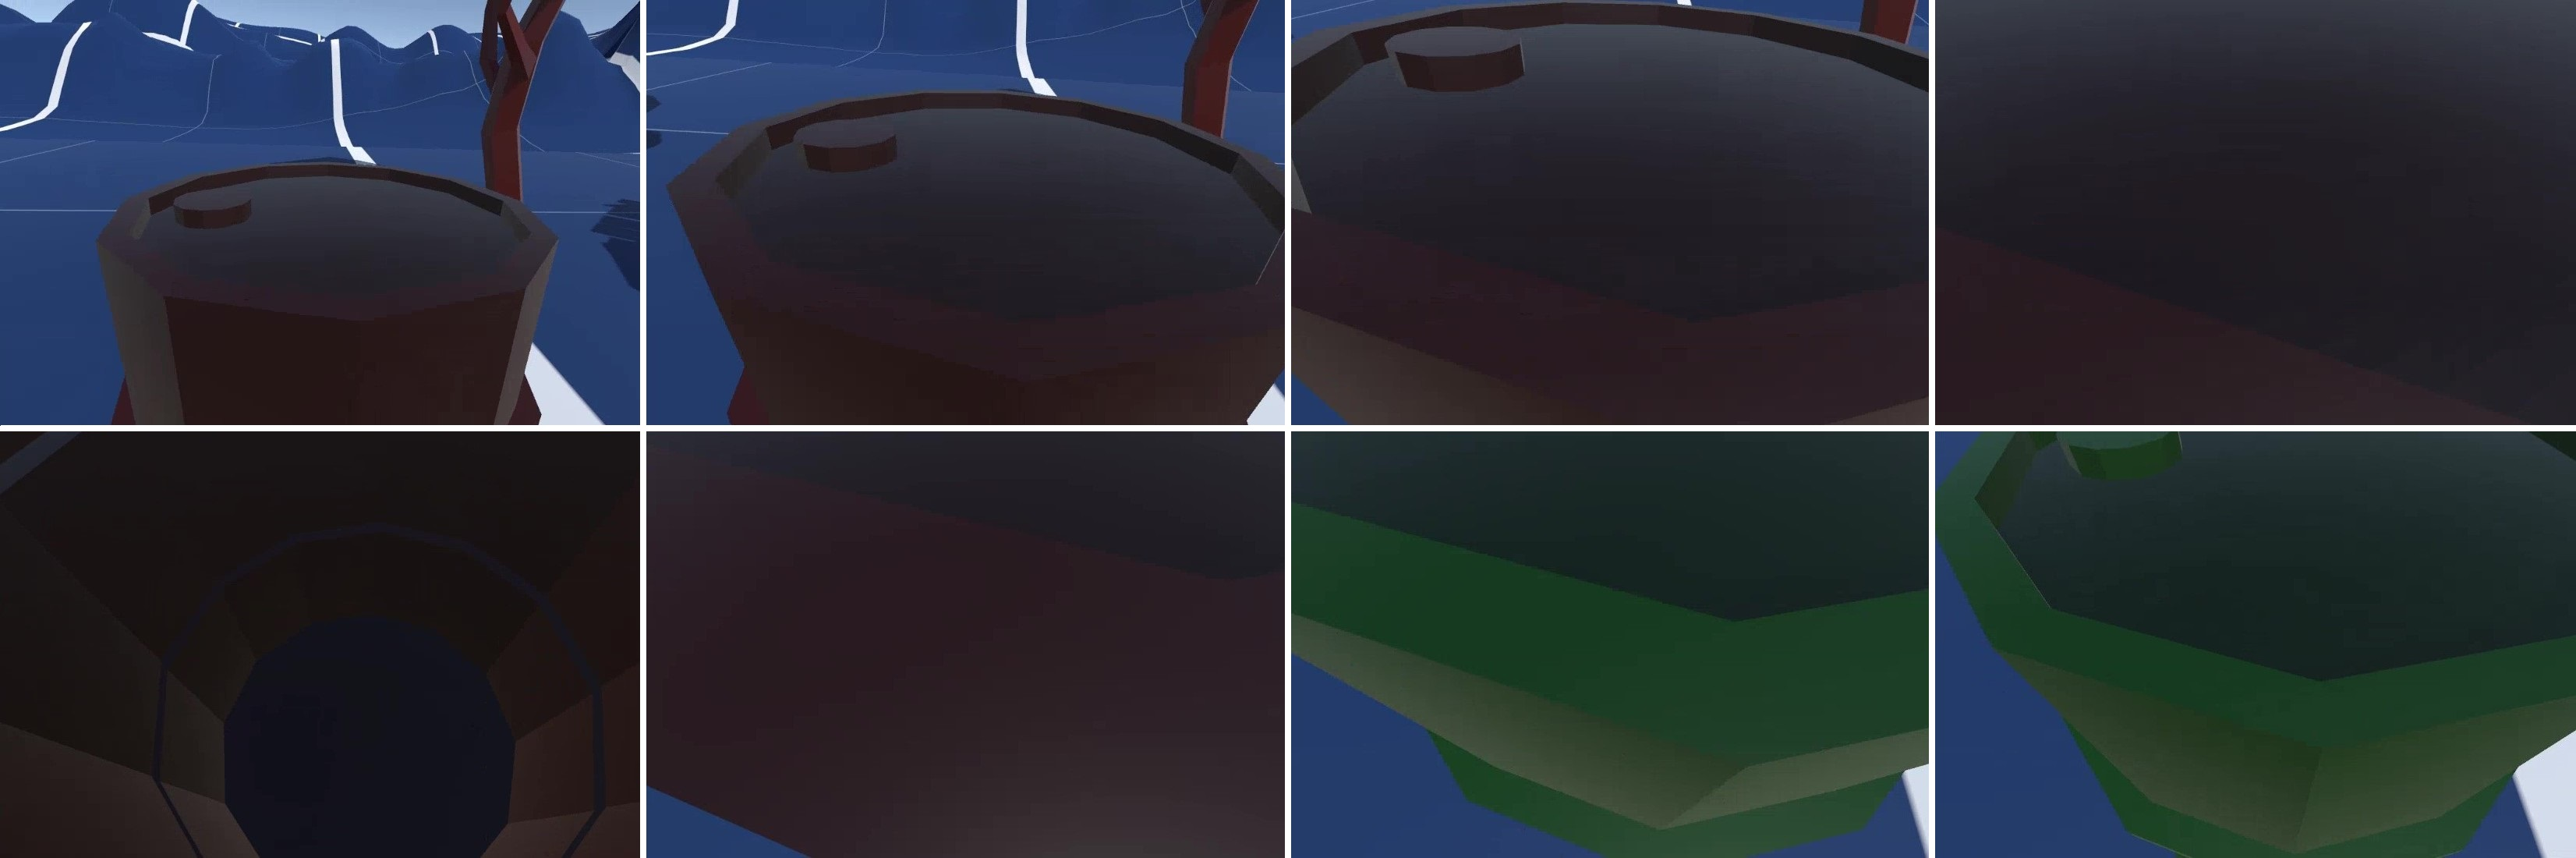
\includegraphics[width=1\textwidth]{img/delayed_implementation.jpg}
\caption{Time slice example of the screen fade technique. When the head collision is detected, the screen slowly fades to black (image source: \cite{SCREENFADE})}
\label{fig:delayedimplementation}
\end{figure}

\begin{figure}[th]
\centering
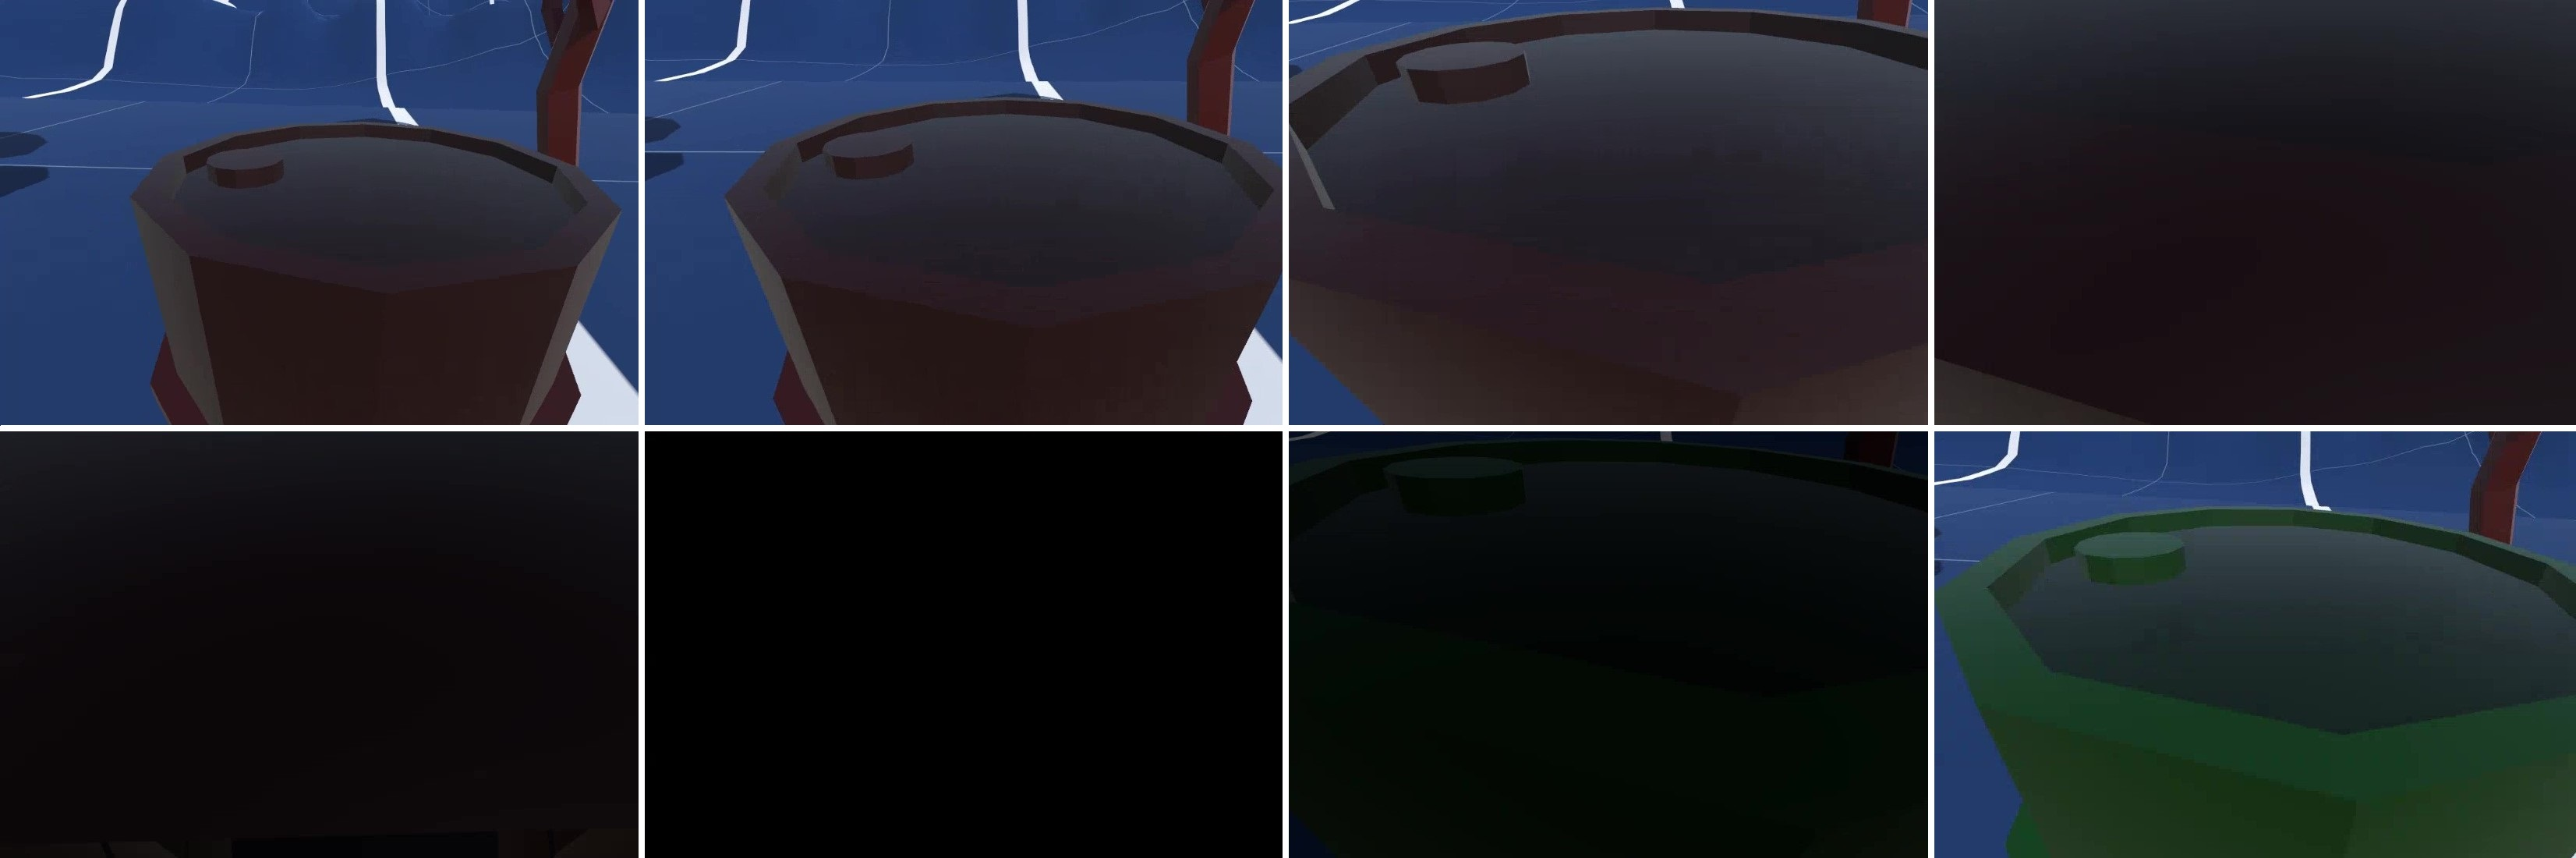
\includegraphics[width=1\textwidth]{img/fade_implementation.jpg}
\caption{Time slice example of the screen fade technique. When the head collision is detected, the screen slowly fades to black (image source: \cite{SCREENFADE})}
\label{fig:fadeimplementation}
\end{figure}

\section{Experiment}

The study employed a within-subject design. The independent variable was the solution to the VR head collisions problem, and it had four levels: screen fade, object fade, camera collider, camera push-back. Due to time constraints, the participants were required to complete the whole experiment with every method in one sitting. The order of tested solutions was assigned randomly with Latin Square counterbalancing. 

\subsection{Equipment}

Opis użytego sprzętu do przeprowadznia eksterymentu (Vive Headset, Vive Controllers, parametry laptopa, średnia liczba FPSów podczas eksperymentu).

\subsection{Participants}

Opis uczestników eksperymentu. Wyniki ankiety demograficznej.

\subsection{Procedure}

Opis przebiegu eksperymentu.